\section{Sparse Regularization}
\label{sec:Sparse Regularization}


\subsection{Point Cloud Consolidation}
\label{subsec:Point Cloud Consolidation}

Point cloud consolidation, known as reconstructing the geometry of a shape from scanned data, is a convenient and direct way to obtain 3D models.
It can be a preprocessing phase for some geometry problem, e.g., surface reconstruction whose result is a mesh object, with functionalities such as denoising, outlier removal, orientation, and redistribution of the input points.
However, even with high-fidelity scanners, a variety of acquisition errors, like noise, outliers, missing data(holes) or registration artifacts, are inevitable in the produced large amount of raw, dense point sets.
Then finding a robust consolidation technique has always been an active researching area.
%The following works are all $\ell_1$ norm based.

\subsubsection{$\ell_1$ median based}
\label{subsubsec:l1 median based}

\begin{figure}[ht]
  \centering
  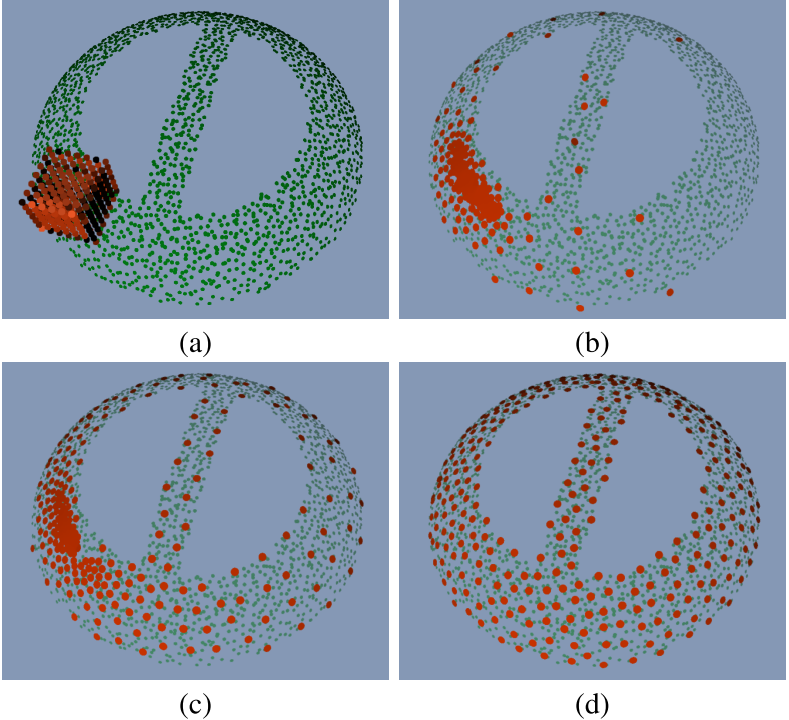
\includegraphics[width=2.0in]{images/L1median}
  \caption{Reconstruction by projection operation. (a). noisy point-set P(green) and an arbitrary point-set Q(red) that will be projected to P to approximate P. (b),(c) are two iterative projection results. (d) is the final projection.}
  \label{fig:L1 median}
\end{figure}

Reconstruction by a projection operator, as shown in Figure~\ref{fig:L1 median}, is to approximate the origin point set(green) by iteratively projecting an arbitrary point set(red) onto itself while removing the noises or outliers.
It has an important virtue: it defines a consistent geometry based on the data points, and provides constructive means to up-sample it.

$\ell_1$ median\cite{brown1983statistical,small1990survey}, closely related to projection operator, is a statistical tool applied globally to multivariate non-parametric point-samples in the presence of noises and outliers.
Briefly, it is a robust global center of an arbitrary set of points.
Given a data set $P=\{p_{j}\}_{j\in J}\subset \mathbb{R}^3$,
the $\ell_1$ median is defined as the point $q$ obtained by minimizing the sum of Euclidean distances to the data points

\small{
\begin{equation}
 \label{eq:L1median}
 q=\arg\min_{x}\left\{ \sum_{j\in J}^{}\|p_{j}-x\| \right\}
\end{equation}
}

\paragraph{(1)}

\cite{lipman2007parameterization} applies this tool locally to constitute a parameterization-free local projection operator(LOP).
Starting with an arbitrary initial point set $X^0=\{ x{_{i}^0}  \}_{i\in I}\subset \mathbb{R}^3$(typically $|X|\ll|P|$, $|\cdot|$ is the number of point set),
LOP computes the target point positions $X$ by performing a fixed-point iteration

\small{
\begin{equation}
 \label{eq:LOP1}
 X^{k+1}=\mathop{\argmin}_{X=\{x_{i}\}_{i\in I}}\{E_1(X^{k},P)+E_2(X^{k})\},\\
\end{equation}
}
\\
where,
\small{
\begin{equation}
 \label{eq:LOP2}
 \begin{split}
 & E_1(X^{k},P)=\sum_{i\in I}^{}\sum_{j\in J}^{}\|x_{i}-p_{j}\|\theta(\|x{_i^k}-p_{j}\|),\\
 & E_2(X^{k})=\sum_{i'\in I}^{}\lambda_{i'}\sum_{i\in I\setminus\{i'\}}^{} \eta(\|x_{i}-x{_{i'}^k}\|)\theta(\|x{_i^k}-x{_{i'}^k}\|).
 \end{split}
\end{equation}
}
\\
The term $E_1$ is in fact a $localized$ version of~(\ref{eq:L1median}) by using a fast-decaying weight function $\theta(r)=e^{-r^2/(h/4)^2}$ with the finite support radius $h$,
and thus it is just $E_1$ that drives the projected points $X$ to approximate the geometry of $P$.
The term $E_2$ keeps the distribution of the points $X$ fair by incorporating local repulsion forces.

To be convenient for the following works, now we give the expression of the solution. Let $\xi{_{ij}^k}=x{_i^k}-p_{j}$ and $\delta{_{ii'}^k}=x{_i^k}-x{_{i'}^k}$, solving~(\ref{eq:LOP1}), the projection for point $x{_i^{k+1}}$ is obtained as

\small{
\begin{equation}
 \label{eq:LOP3}
 x{_i^{k+1}}=F_1(x{_i^k},P)+F_2(x{_i^k},X{_i^{'}})
\end{equation}
}
\\
where,
\small{
\begin{equation}
 \label{eq:LOP4}
 \begin{split}
 & F_1(x{_i^k},P)=\sum_{j\in J}^{}p_{j}\frac{\alpha{_{ij}^k}}{\sum_{j\in J}^{}\alpha{_{ij}^k}},\\
 & F_2(x{_i^k},X{_i^{'}})=\mu\sum_{{i'}\in I\setminus\{i\}}^{}\delta{_{ii'}^k}\frac{\beta{_{ii'}^k}}{\sum_{{i'}\in I\setminus\{i\}}^{}\beta{_{ii'}^k}},\\
 & \alpha{_{ij}^k}=\frac{\theta(\|\xi{_{ij}^k}\|)}{\|\xi{_{ij}^k}\|},
   ~\beta{_{ii'}^k}=\frac{\theta(\|\delta{_{ii'}^k}\|)|\eta'(\|\delta{_{ii'}^k}\|)|}{\|\delta{_{ii'}^k}\|}.
 \end{split}
\end{equation}
}

Intuitively, LOP distributes the points by approximating their $\ell_1$ median to achieve robustness to outliers and data noises without any local orientation information nor a local manifold assumption.
But, also because of the use of the local density parameter $h$, it may not work well when the distribution of the input points is highly non-uniform and can fail to converge.

\paragraph{(2)}

Like\cite{lipman2007parameterization}, many consolidation methods try to obtain the resulted geometry object
without estimation of normals due to the unreliability resulting from the noisy data as oppose to the fact that
oriented normals at the points play a critical role in geometry reconstruction.

To achieve a better normal estimation that requires the sampling points to be uniformly distributed,
\cite{huang2009consolidation} incorporates locally adaptive density weights into LOP, resulting in a new consolidation technique WLOP, to address the non-uniform distribution problem while taking advantage of the success of LOP in denoising and outlier removal.

They define the weighted local densities for each point $p_{j}$ in $P$ and $x_{i}$ in $X$ during the $k$th iteration by $v_{j}=1+\sum_{j'\in J\setminus\{j\}}^{}\theta(\|p_{j}-p_{j'}\|)$ and $w{_i^k}=1+\sum_{i'\in I\setminus\{i\}}^{}\theta(\|\delta{_{ii'}^k}\|)$, the term $F_1$ and $F_2$ in~(\ref{eq:LOP4}) finally becomes

\small{
\begin{equation}
 \label{eq:WLOP}
 \begin{split}
 & F_1(x{_i^k},P)=\sum_{j\in J}^{}p_{j}\frac{\alpha{_{ij}^k}/v_{j}}{\sum_{j\in J}^{}(\alpha{_{ij}^k}/v_{j})}\\
 & F_2(x{_i^k},X{_i^{'}})=\mu\sum_{{i'}\in I\setminus\{i\}}^{}\delta{_{ii'}^k}\frac{w{_{i'}^k}\beta{_{ii'}^k}}{\sum_{{i'}\in I\setminus\{i\}}^{}(w{_{i'}^k}\beta{_{ii'}^k})},
 \end{split}
\end{equation}
}
\\
The weighted local density $v$ in $F_1$ relaxes the attraction of point clusters and
repulsion force in dense areas is strengthened by the local density $w$ in $F_2$.

Here, the obtained uniformly distributed point set can largely improve the reliability of normal initialization for a second normal estimation phase.
Practically, due to the high computational effort, it may not be a preferable choice to use this consolidation technique as a preprocessing method for surface reconstruction, even though some high quality surface can be reconstructed.


\paragraph{(3)}
In LOP/WLOP, the majority of the time is spent on the evaluation of the attractive forces from all points in $P$,
so \cite{preiner2014CPF} efficiently reduce the set $P$ of unordered input points to a much more compact mixture of Gaussians $\mathcal{M}=\{w_{s},\Theta_{s}\}$ that reflects the density distribution of the points.
That is, $\mathcal{M}$ defines a probability density function(pdf) as a weighted sum of $|\mathcal{M}|$ Gaussian components

\small{
\begin{equation}
 \label{eq:CLOP1}
 f(\mathbf{x}|\mathcal{M})=\sum_{s}^{}w_{s}g(\mathbf{x}|\Theta_{s}),
\end{equation}
}
\\
where the $\Theta_{s}=(\mu_{s},\sum_{s}^{})$ are the Gaussian parameters,
$w_{s}$ are their corresponding convex weights, and
$g$ denotes the $d$-variate Gaussian pdf.
%with $g(\mathbf{x}|\mu,\sum)=|2\pi\sum_{}^{}|^{-\frac{1}{2}}e^{-\frac{1}{2}(\mathbf{x}-\mu)^{T}\sum_{}^{-1}(\mathbf{x}-\mu)}$.

They define a $continuous$ $\mathcal{F}_1$ corresponding to $F_1$ in~(\ref{eq:LOP4}) by the convex sum over the internal attraction of each single Gaussian, with convex weights $w_s$ accounting for the Gaussian's relative point mass:

\small{
\begin{equation}
 \label{eq:CLOP2}
 \mathcal{F}_1(q,\mathcal{M})=\sum_{s}^{}w_s\int_{\mathbb{R}^3}^{}
 \frac{\mathbf{x}g(\mathbf{x}|\Theta_{s})\alpha(\mathbf{x})}
 {\sum_{s'}^{w_{s'}}\int_{\mathbb{R}^3}^{}g(\mathbf{x'}|\Theta_{s'})\alpha(x')d\mathbf{x}'}
 d\mathbf{x},
\end{equation}
}
\\
and the final \textbf{closed form} is expressed as
\small{
\begin{equation}
 \label{eq:CLOP3}
 \mathcal{F}_1(q,\mathcal{M})=\frac{\sum_{s}^{}\sum_{k}^{}\int_{\mathbb{R}^3}^{}\mathbf{x}\widehat{\Omega}_{sk}(\mathbf{x})d\mathbf{x}}
 {\sum_{s}^{}\sum_{k}^{}\int_{\mathbb{R}^3}^{}\widehat{\Omega}_{sk}(\mathbf{x})d\mathbf{x}}
 =\frac{\sum_{s,k}^{}w_{sk}\mu_{sk}}
 {\sum_{s,k}^{}w_{sk}}
\end{equation}
}
\\
changing the convex sum of 3D points $p_{j}$~(\ref{eq:LOP2}) into a convex combination of the product Gaussians' means $\mu_{sk}$ with weights $w_{sk}$.
Figure~\ref{fig:L1 median consolidation} shows the results of these three methods.

This continuous method is up to 7 times faster than an optimized GPU implementation of LOP/WLOP, and achieves interactive frame rates for moderately sized point clouds though it can not automatically get the best choice of the parameters for different point set.

\begin{figure}[ht]
  \centering
  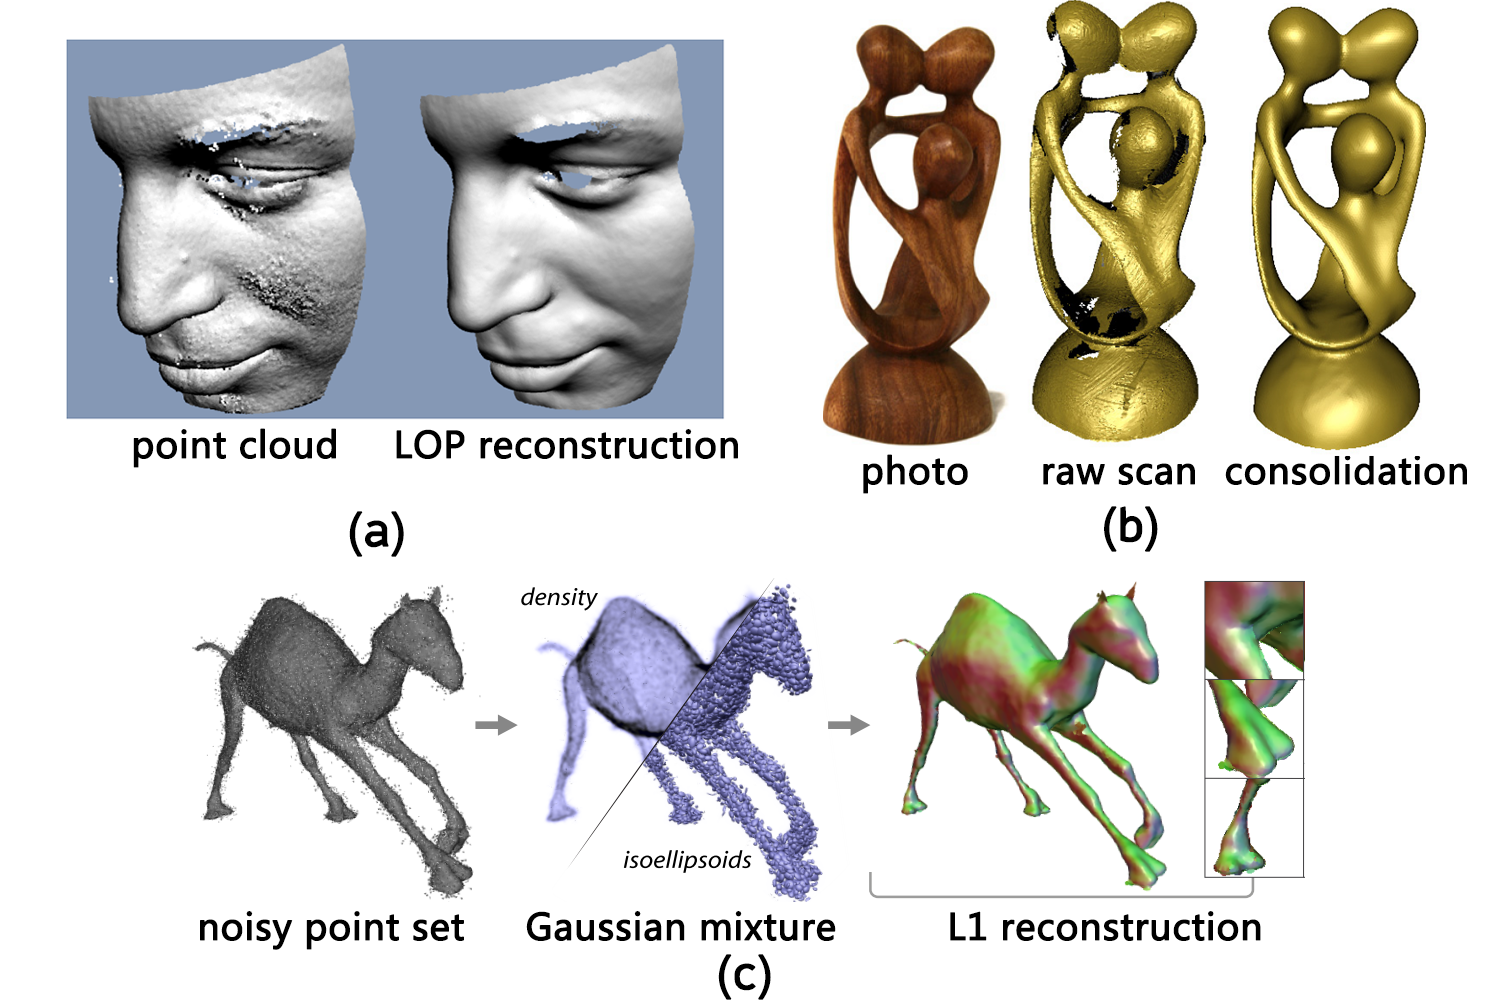
\includegraphics[width=2.5in]{images/reconstruction_L1}
  \caption{Sparse regularization: point cloud consolidation. (a): LOP\cite{lipman2007parameterization}. (b): WOLP\cite{huang2009consolidation}. (c): continuous WLOP\cite{preiner2014CPF}.}
  \label{fig:L1 median consolidation}
\end{figure}


\subsubsection{$\ell_1$ regression based}
Due to the robustness to noises and outliers of $\ell_1$ norm,
\cite{mustafa2014subdivision} develops an $\ell_1$ regression based subdivision algorithm for curve and surface fitting, 
where the size of target point cloud is largely more than that of origin data in contrast to the previous consolidation works.

For curve fitting, they try to find the best fit straight line $f(x)=\beta_1+\beta_2 x$ with observations$(x_r=r, f_r),r=-n+1,\cdots,n$.
The $\ell_1$ regression optimization is simply formulated as

\small{
\begin{equation}
 \label{eq:subdivision}
 \begin{split}
 &\beta_1, \beta_2 = \arg \min_{\beta_1,\beta_2\in\mathbb{R}}  \sum_{r=-n+1}^{n}  | f_r - (\beta_1 + \beta_2 r) |\\
 &~~~~~~~~=\arg \min_{\beta_1,\beta_2\in\mathbb{R}} F(\beta_1,\beta_2),
 \end{split}
\end{equation}
}
\\
because of the lack of differentiability, they regularize $F$ with a family of convex functional $F_{\delta}$, $\delta>0$,

\small{
\begin{equation}
 \label{eq:subdivision regularization}
 \begin{split}
 &F_{\delta}(\beta_1, \beta_2) = \sum_{r=-n+1}^{n}  h_{\delta}( f_r -\beta_1 - \beta_2 r),~\textrm{where}\\
 &h_{\delta}( f_r -\beta_1 - \beta_2 r) = [( f_r -\beta_1 - \beta_2 r)^2+\delta]^{1/2}
 \end{split}
\end{equation}
}
\\
then for a given $\delta$, the solution of (\ref{eq:subdivision}) is approximated by $\beta_{1,\delta}$ and $\beta_{2,\delta}$.
By substituting optimum $\beta_{1,\delta}$, $\beta_{2,\delta}$ into $f(x)$ and evaluating this function at 1/4 and 3/4,
the closed form of $\ell_1$ scheme for curve fitting is obtained.

With the closed form, $\ell_1$ scheme $D_{2n}$ firstly iteratively assigns weights to only $2n$ local initial points,
then gets the final fitting result(e.g.,Figure~\ref{fig:subdivision}) through subdivision rule for locations of vertices of the new mesh
and topological rule for size of added vertices and their connectivity.


\begin{figure}[ht]
  \centering
  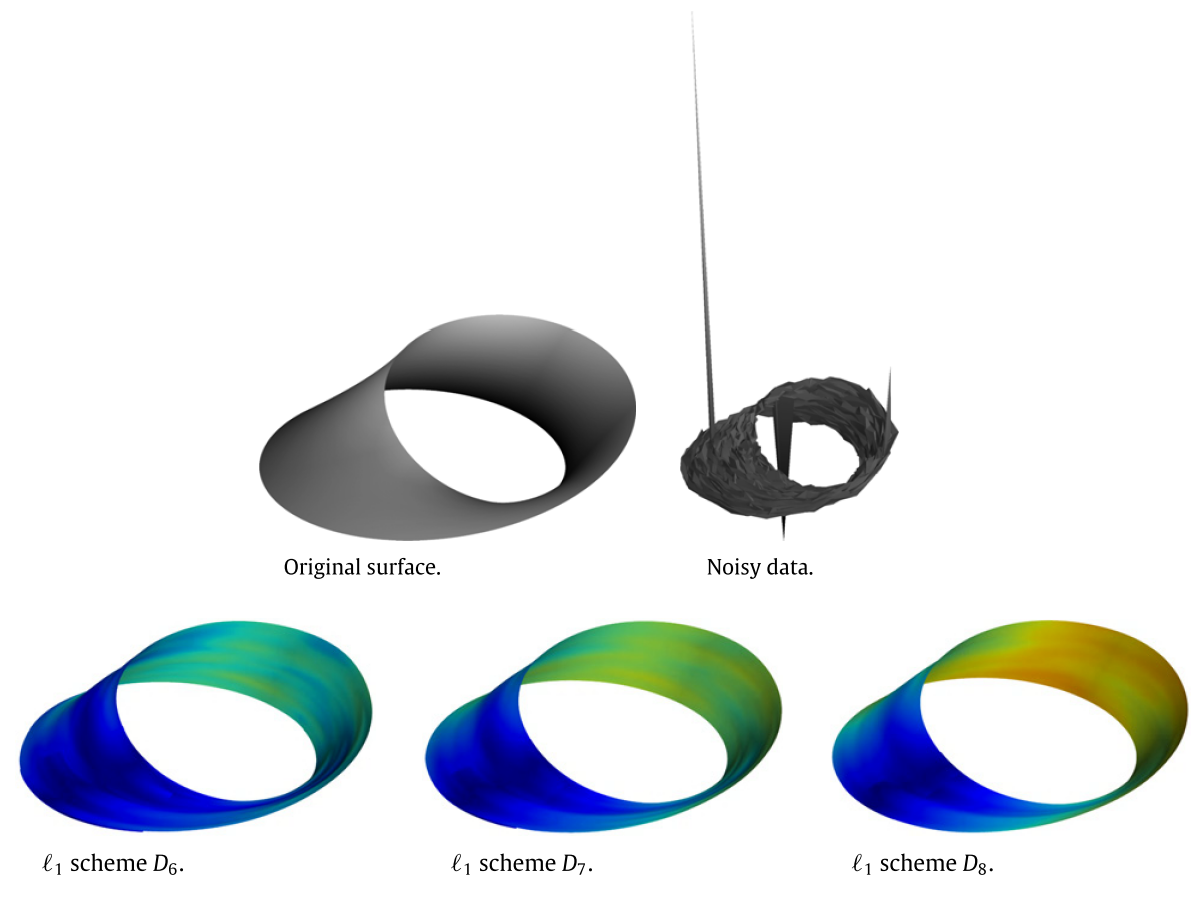
\includegraphics[width=2.5in]{images/subdivision}
  \caption{Sparse regularization: $\ell_1$ based subdivision\cite{mustafa2014subdivision}. Parametric surface reconstructed by $\ell_1$ scheme from highly noisy parametric data with outliers.}
  \label{fig:subdivision}
\end{figure} 